\documentclass{jps-cp}
\usepackage{txfonts} %Please comment out this line unless the txfonts package is availabe in your LaTeX system.
\usepackage{url}
\usepackage{multirow}
\usepackage{array, booktabs}
\usepackage{wrapfig}

\makeatletter
\newcommand{\figcaption}[1]{\def\@captype{figure}\caption{#1}}
\newcommand{\tblcaption}[1]{\def\@captype{table}\caption{#1}}

\title{New analysis method of TPC data using neural network}

\author{
  Takanobu \textsc{Doi}$^{1}$, Takahiro \textsc{Kawabata}$^{2}$, Tatsuya \textsc{Furuno}$^{3}$,
  Yuki \textsc{Fujikawa}$^{1}$, Kento \textsc{Inaba}$^{1}$, Motoki \textsc{Murata}$^{3}$,
  Shintaro \textsc{Okamoto}$^{1}$ and Akane \textsc{Sakaue}$^{1}$}

\inst{
  $^{1}$Department of Physics, Kyoto University, Kyoto, Kyoto 606-8502, Japan \\
  $^{2}$Department of Physics, Osaka University, Toyonaka, Osaka 540-0043, Japan \\
  $^{3}$Research Center for Nuclear Physics, Osaka University, Ibaraki, Osaka 567-0047, Japan }

\email{doi.takanobu.68x@st.kyoto-u.ac.jp}

\recdate{2019/8/4} % Write received date here

\abst{
  TPC を用いた実験では荷電粒子の飛跡を測定することができる。
  TPC では3次元的な荷電粒子の飛跡を2次元平面に射影した画像として得られるので、
  データの解析には画像解析を行う必要がある。
  従来はHough 変換を用いてデータの解析を行って来たが、
  この方法を用いた解析には多くの労力を要する。
  近年、画像データの認識にはニューラルネットワークが注目されている。
  本研究では、新しくニューラルネットワークを用いた解析方法の開発を行った。
  新しく開発した手法を用いることで、従来の方法と比較して高速に解析できるようになった。
} % Write abstract here

\kword{neural networks, convolutional neural networks,
  TPC, active target, MAIKo TPC} % Write keywords here

\begin{document}
\maketitle

\section{Introduction}
近年、荷電粒子の飛跡を測定する検出器としてTime Projection Chamber (TPC) が
広く用いられている。
我々は不安定核実験のためにMicro Pixel Chamber ($\mu$-PIC)~\cite{mupic} (Fig. \ref{fig:uPIC}) 
を用いた
Mu-Pic based Active target for Inverse Kinematics . (MAIKo) TPC~\cite{MAIKo} (Fig. \ref{fig:MAIKo}) を開発した。
TPC は検出器にガスを充填しておき、荷電粒子がガス中を通過するときに発生する
電子をドリフト電場により読み出し面にドリフトさせる
(Fig. \ref{fig:MAIKo} 中では下向きに移動させる) ことで飛跡を検出する。
$\mu$-PIC は2方向の直交する読み出しストリップを持つので、
電子が到達したx, z座標を決定できる。
また、電子が到達するまでのドリフト時間により、
飛跡から読み出し面までの距離 (y座標) を決定することが出来る。
x, y, zの座標が決定できるので、飛跡を3次元的に再構成することが出来る。

\begin{figure}
  \centering
  \begin{minipage}{0.4\columnwidth}
    \centering
    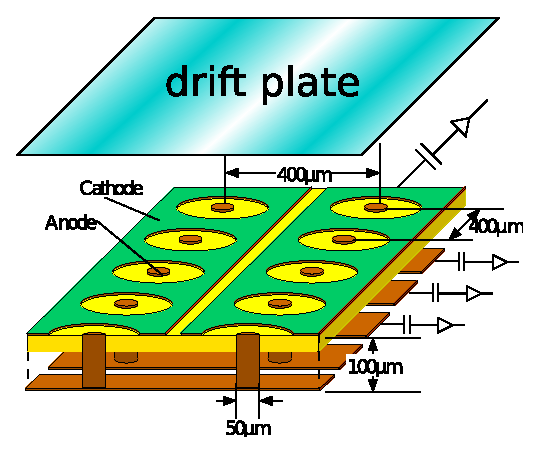
\includegraphics[clip, width=0.9\columnwidth]{eps/upic_struc.eps}
    \caption{$\mu$-PIC の構造}
    \label{fig:uPIC}
  \end{minipage}
  \hfill
  \begin{minipage}{0.4\columnwidth}
    \centering
    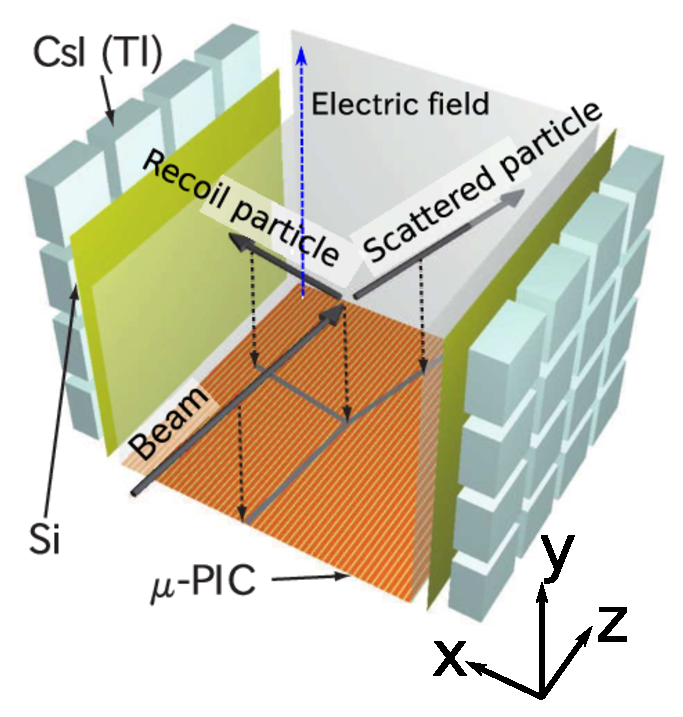
\includegraphics[clip, width=0.9\columnwidth]{eps/MAIKo.eps}
    \caption{MAIKo TPC の外観。}
    \label{fig:MAIKo}
  \end{minipage}
\end{figure}

この検出器では検出ガスを実験の標的として用いる (アクティブ標的) 。
散乱が検出器内部で起こるため、大立体角で低エネルギー粒子の測定を行うことが可能となる。
広く標的ガスとして用いられるのは $\rm{He}$ や $\rm{H}_{2}$であるが、
これらのガスは放電耐性が低いので、
通常は放電耐性の高い $\rm{CO}_{2}$ やイソブタンをクエンチングガスとして
混入させてTPC を運用する。
このとき、クエンチングガスからの散乱は背景事象となる。
近年、大阪大学核物理研究センター (RCNP) において、
MAIKo TPC を用いた${}^{10}\rm{C}$と${}^{4}\rm{He}$の非弾性散乱の測定が初めて行われた。
この実験では標的ガスとして$\rm{He}$、クエンチングガスとして$\rm{CO}_{2}$を
96:4 の割合で混合して用いた。

荷電粒子の飛跡はビーム軸に平行な面に射影された画像 (anode image) と
ビーム軸に垂直な面に射影された画像 (cathode image) の2つの画像として取得される。
$\mu$-PIC のストリップは400 $\mu$m 間隔で256 本あり、
信号波高の時間変化は100 MHz で1024 samples 測定されるので、
取得される画像の解像度は256 $\times$ 1024 pixels となる。
Figs. \ref{fig:true} and \ref{fig:false} はRCNPで行われた実験で取得された
データの一例である。
Fig. \ref{fig:true} は$\rm{He}$ガスと散乱した事象、
Fig. \ref{fig:false} はクエンチングガスと散乱した事象である。

散乱実験では、散乱粒子のエネルギーと放出角度を決定する必要がある。
散乱粒子のエネルギーは散乱粒子がガス中で停止するまでの飛跡の長さから、
放出角度は散乱前後の粒子の飛跡から決定することが出来る。
飛跡情報の抽出を行うためには
\begin{itemize}
\item 標的との散乱事象と背景事象との選別
\item 飛跡の長さや方向などの物理的情報の抽出
\end{itemize}
の大きくわけて2つの解析が必要になる。

\begin{figure}
  \centering
  \begin{minipage}{0.4\columnwidth}
    \centering
    \includegraphics[clip, width=0.9\columnwidth]{eps/true.eps}
    \caption{${}^{10}\rm{C}+{}^{4}\rm{He}$の散乱事象}
    \label{fig:true}
  \end{minipage}
  \begin{minipage}{0.4\columnwidth}
    \centering
    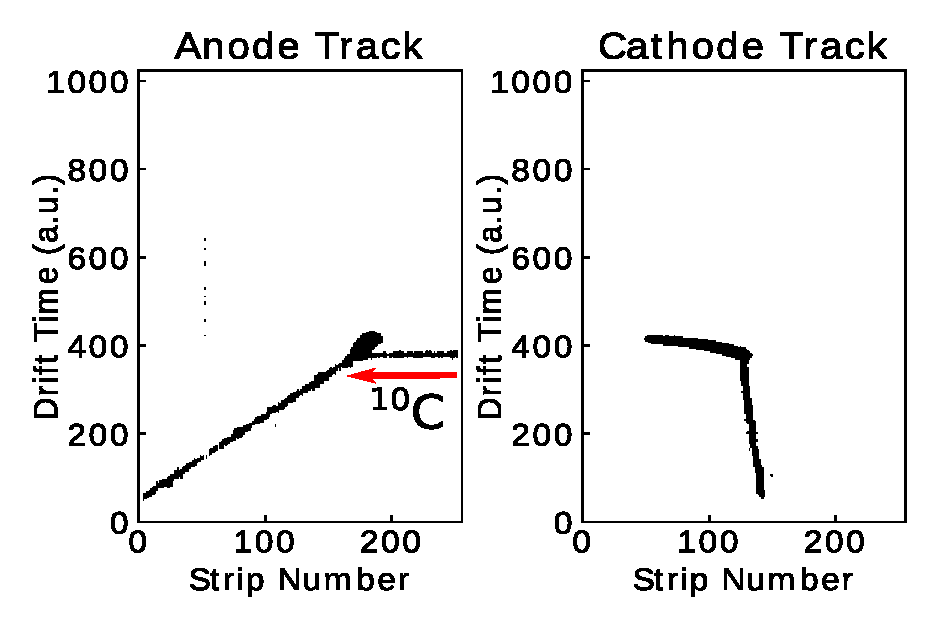
\includegraphics[clip, width=0.9\columnwidth]{eps/false.eps}
    \caption{${}^{10}\rm{C}$とクエンチガスとの散乱事象}
    \label{fig:false}
  \end{minipage}
\end{figure}

Figs. \ref{fig:true} and \ref{fig:false} のような画像データに対して、
事象の選別や飛跡情報の抽出には多くの労力が必要となる。
そこで、我々は近年画像認識において多くの成果を出している
ニューラルネットワークを用いることで、
より高速な解析を行うことが出来る解析方法の開発を行った。

\section{Conventional analysis method}
従来は、得られたデータから背景事象の除去を行うのに、
画像中の直線を抽出する手法の1つである
Hough 変換を用いたアルゴリズムによって行ってきた。
Hough 変換を行うことで画像に含まれる飛跡上の点は、
原点からの距離 ($r$) と傾き ($\theta$) の
2つの軸を持つパラメータ空間 (Hough 空間) における曲線へ変換される。
元の画像における直線上の点はすべて同じ $r$ と $\theta$ を共有するので、
このパラメータ空間において複数の曲線が交わる点を求めれば
$r$ と $\theta$が一意に決定され、元の画像における直線
を抽出することができる。
抽出した直線に沿って端点を探すことで、画像に含まれる飛跡の方向と長さを決定することができる。
決定された飛跡の長さや角度、本数、配置に対して多くの条件を課すことによって、
$\rm{He}$との散乱事象を選別することが出来る。
しかし、この条件を設定するには複雑な分岐を必要とし、
多くのパラメータを導入しなければならない。
そのため、パラメータの最適化や画像識別に多くの時間を必要とする。
さらに、選別された事象における$\rm{He}$の飛跡の長さや角度から、
散乱角とエネルギーを決定することが出来る。

パラメータの最適化には100 CPU を使用して約1日かかり、
その後の識別には1 eventあたり1秒かかった。
この手法による識別能力の評価には、画像データを人間が目で見て
散乱事象もしくは背景事象と判断した3000イベントを評価用データとして用いて行った。
全事象のうち、散乱事象または背景事象の区別を正しく判断することが
出来た事象数の割合を正解率としたとき、この従来型の解析手法では89\%の正解率であった。

\section{New analysis method}

%\begin{wrapfigure}{r}{15zw}
%  \centering
%  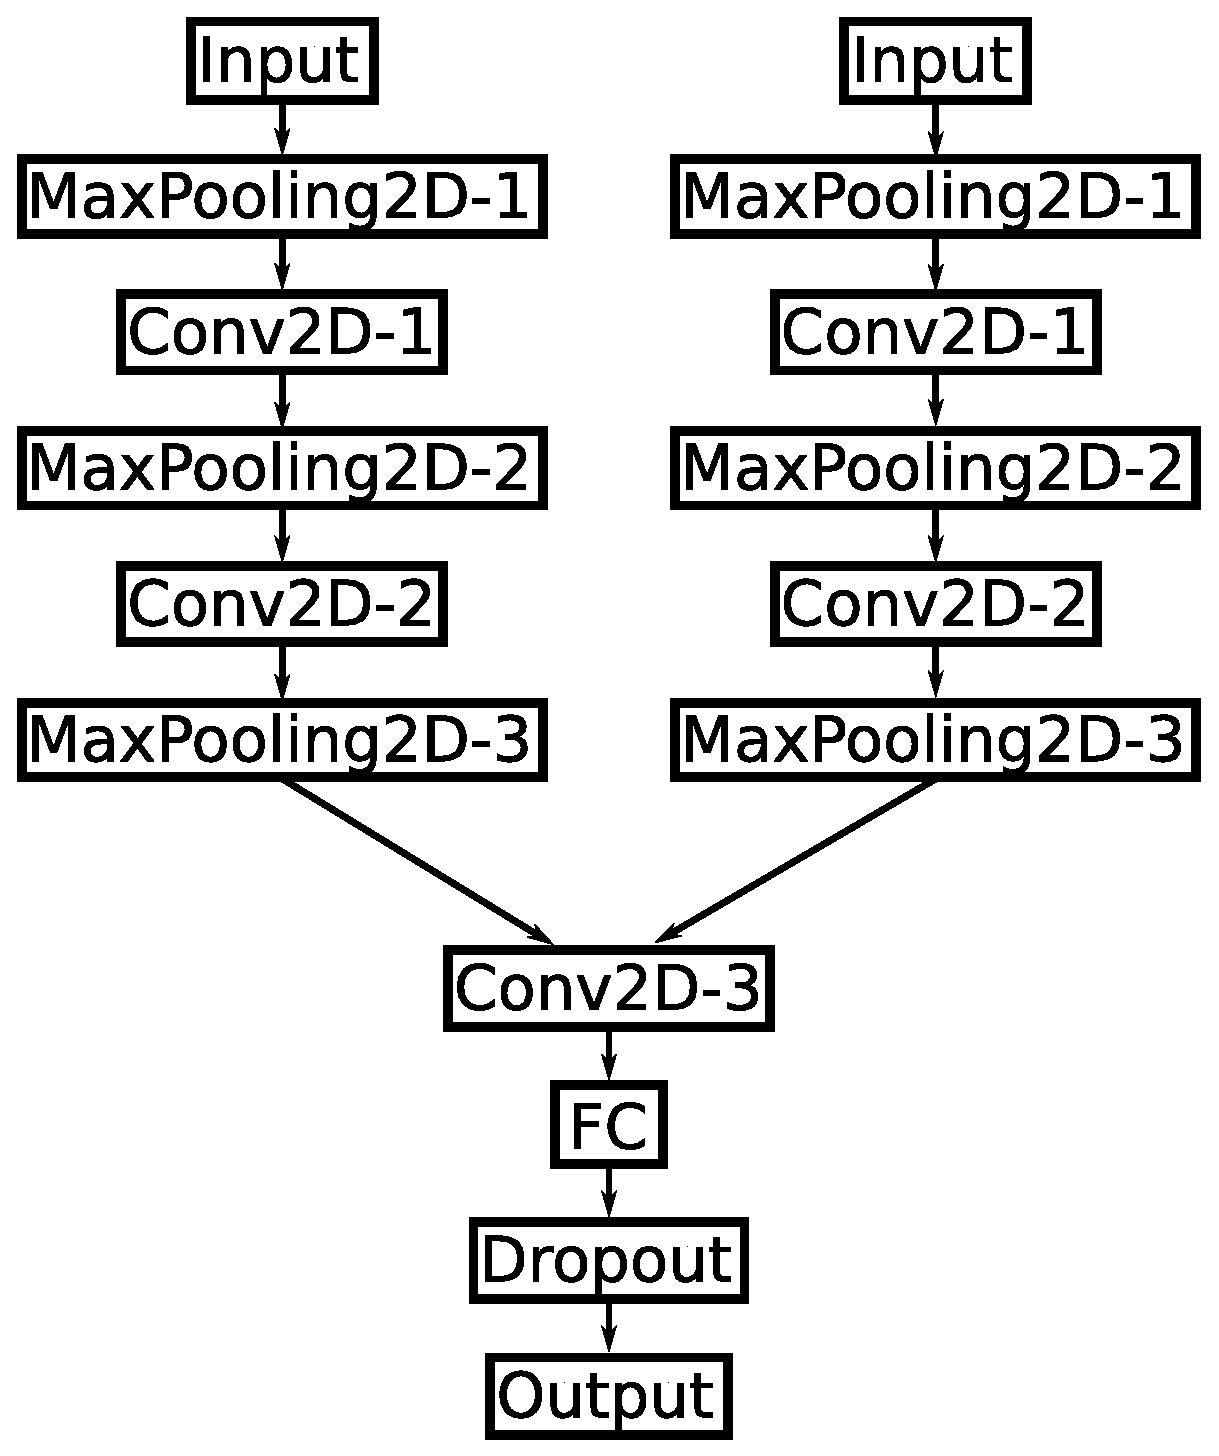
\includegraphics[clip, width=15zw]{eps/event_selection.eps}
%  \caption{データの選別を行うためのニューラルネットワーク}
%  \label{fig:selection}
%\end{wrapfigure}

従来手法では識別に複雑な分岐条件や多くの計算機パワー
が必要になるという問題点があった。
そこで、我々は近年注目されているニューラルネットワークを用いることで、
これらの問題点を克服する新しい解析方法の開発を試みた。
ニューラルネットワークを用いることで、複雑な条件分岐を導入することなく、
直線の位置、角度などの従来の解析手法ではまとめて扱うことの難しい
多くの特徴量を同時に考慮した画像識別が可能になるかもしれない。
また、ニューラルネットワークは一度構築するとその後は短時間で画像識別を行うことができる。
このようなニューラルネットワークの特徴を活かすことで、
従来のアルゴリズムでは実現が難しかった高い精度と短い識別時間を実現することが期待される。

%\begin{wrapfigure}{r}{15zw}
%  \centering
%  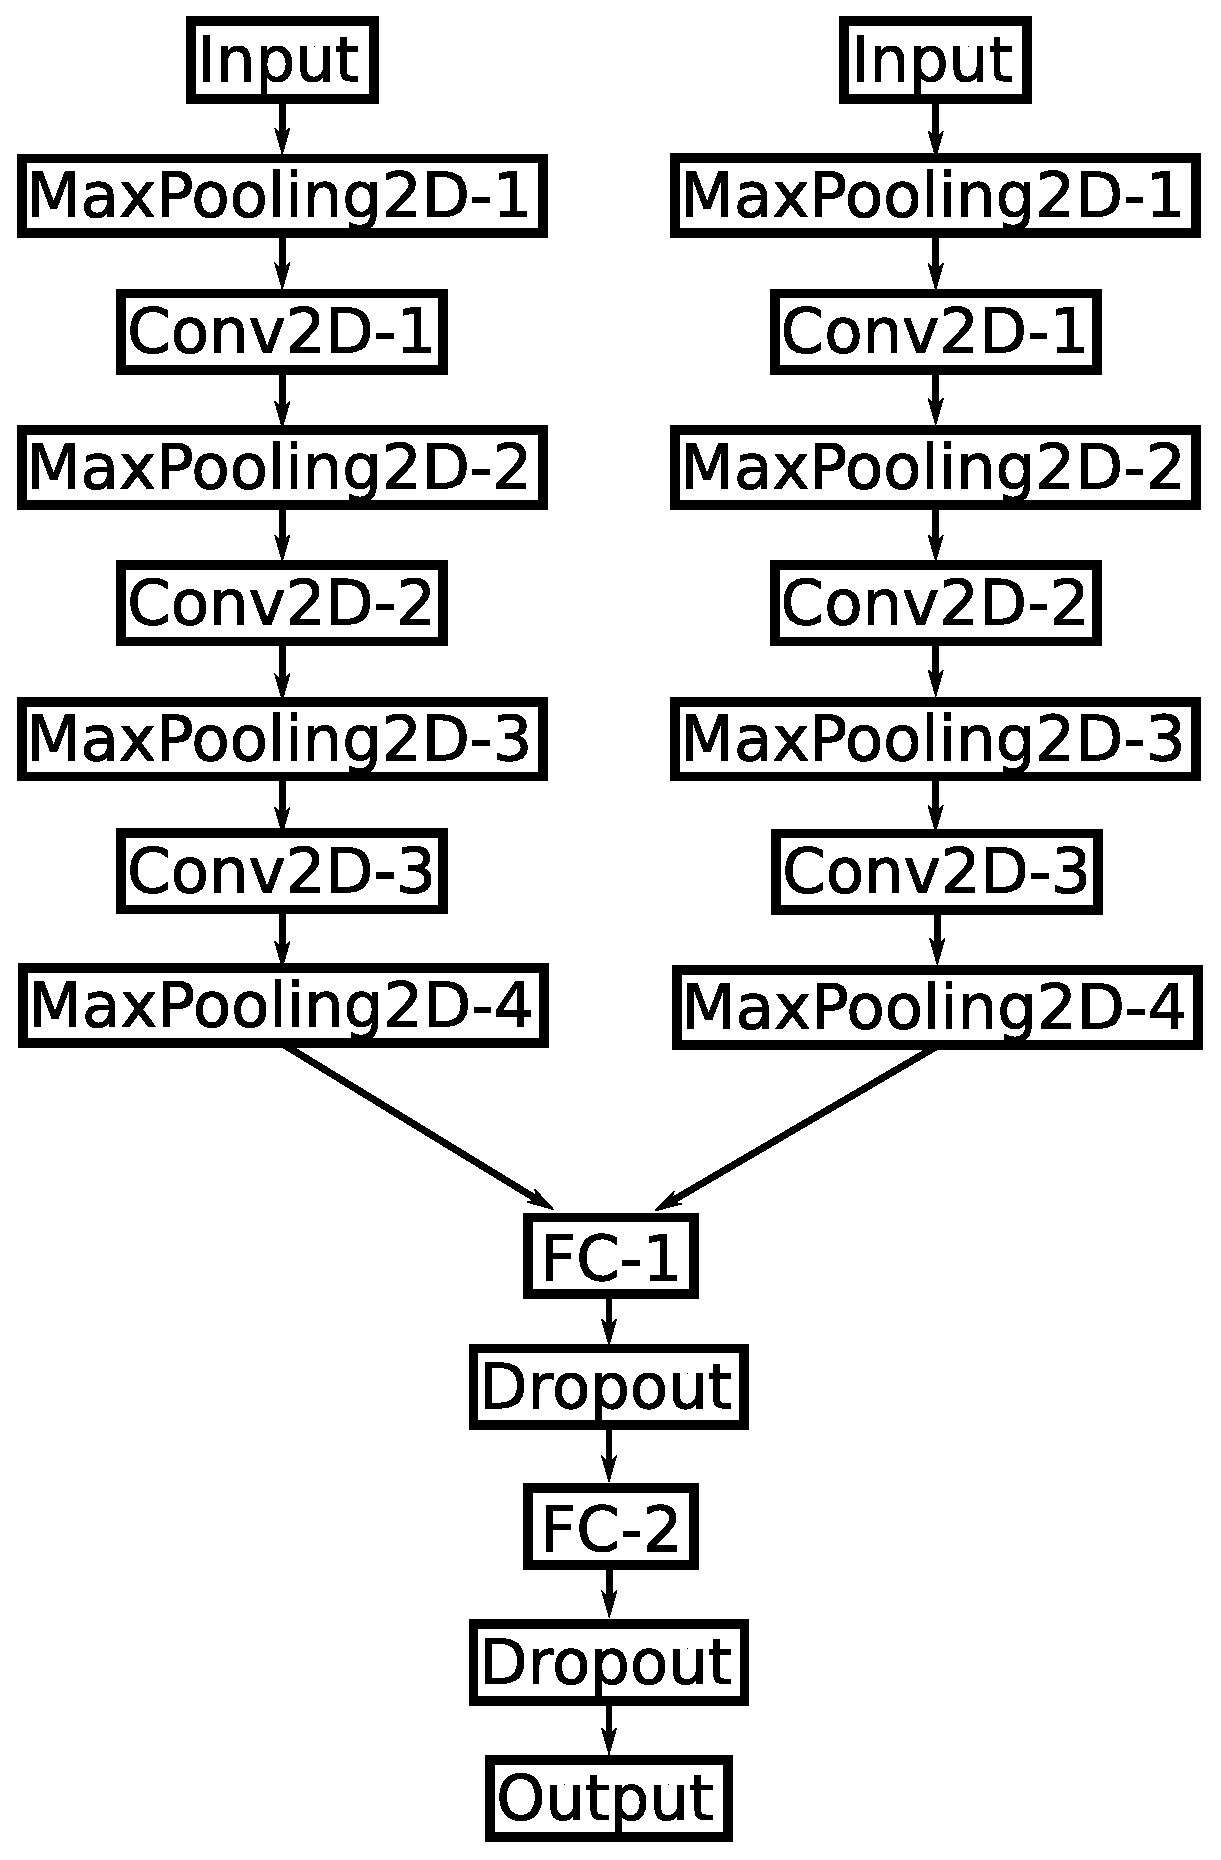
\includegraphics[clip, width=15zw]{eps/point_detection.eps}
%  \caption{画像から情報を抽出するためのニューラルネットワーク}
%  \label{fig:extraction}
%\end{wrapfigure}
\begin{figure}
  \centering
  \begin{minipage}{0.4\columnwidth}
    \centering
    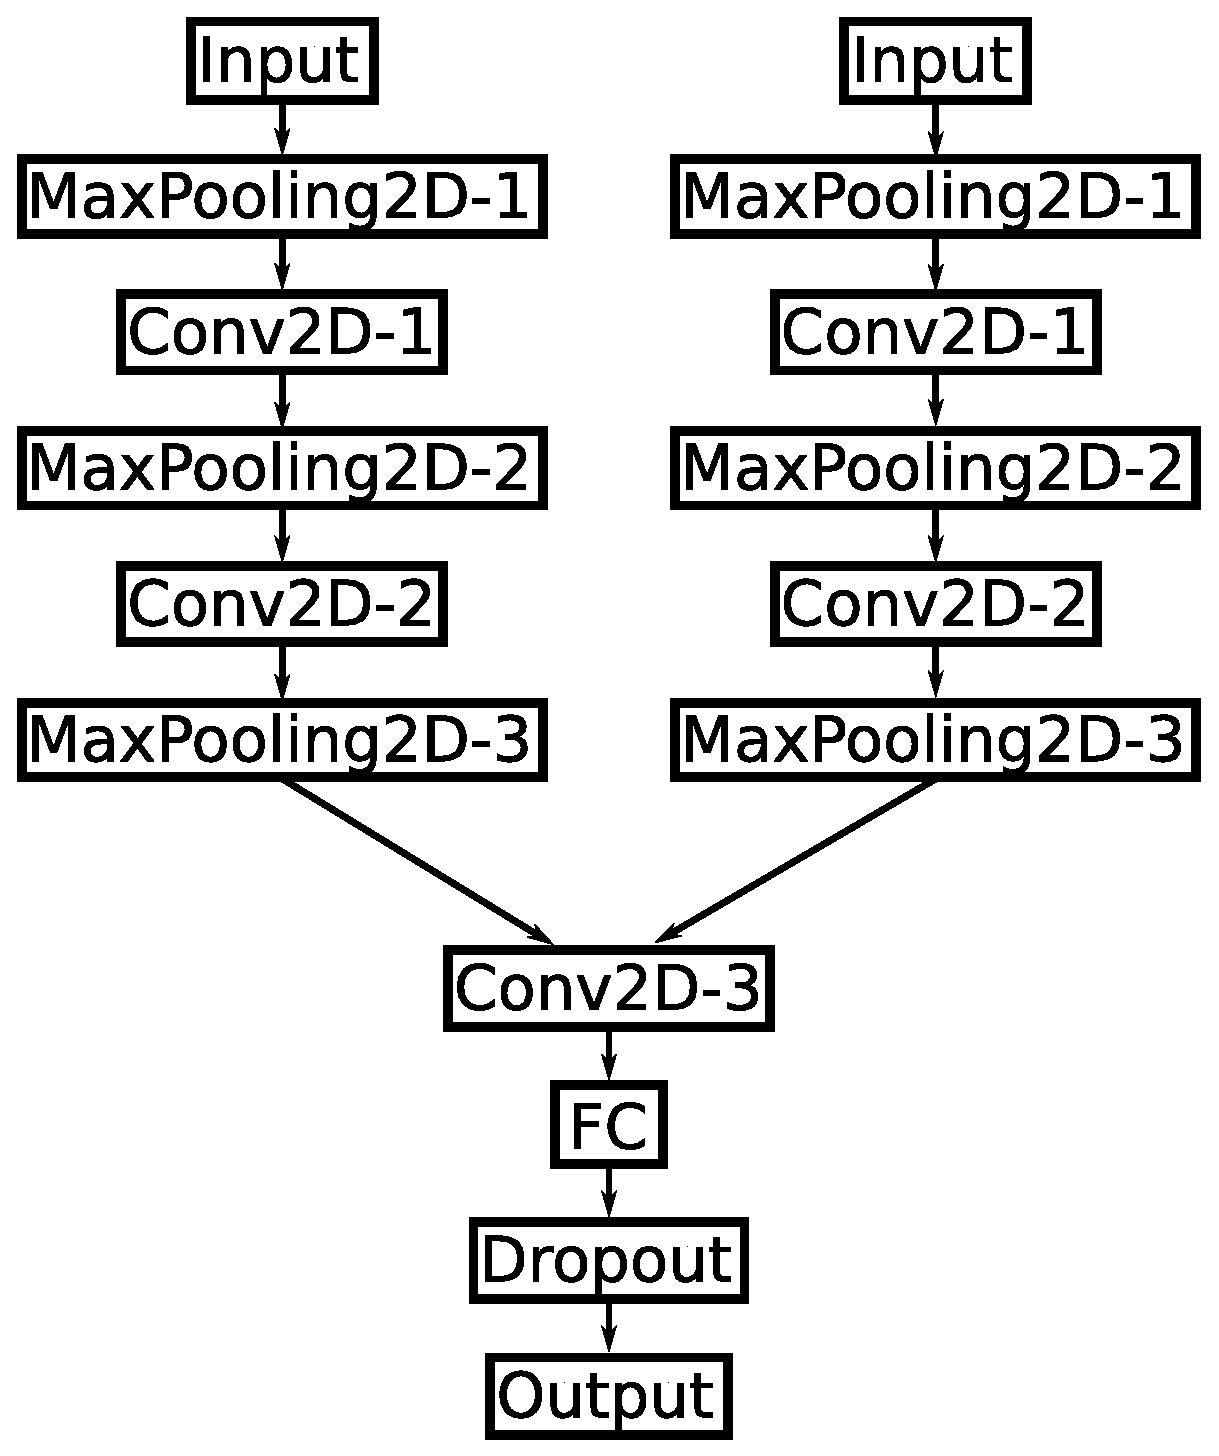
\includegraphics[clip, width=0.9\columnwidth]{eps/event_selection.eps}
    \caption{データの選別を行うためのニューラルネットワーク}
    \label{fig:selection}
  \end{minipage}
  \hfill
  \begin{minipage}{0.4\columnwidth}
    \centering
    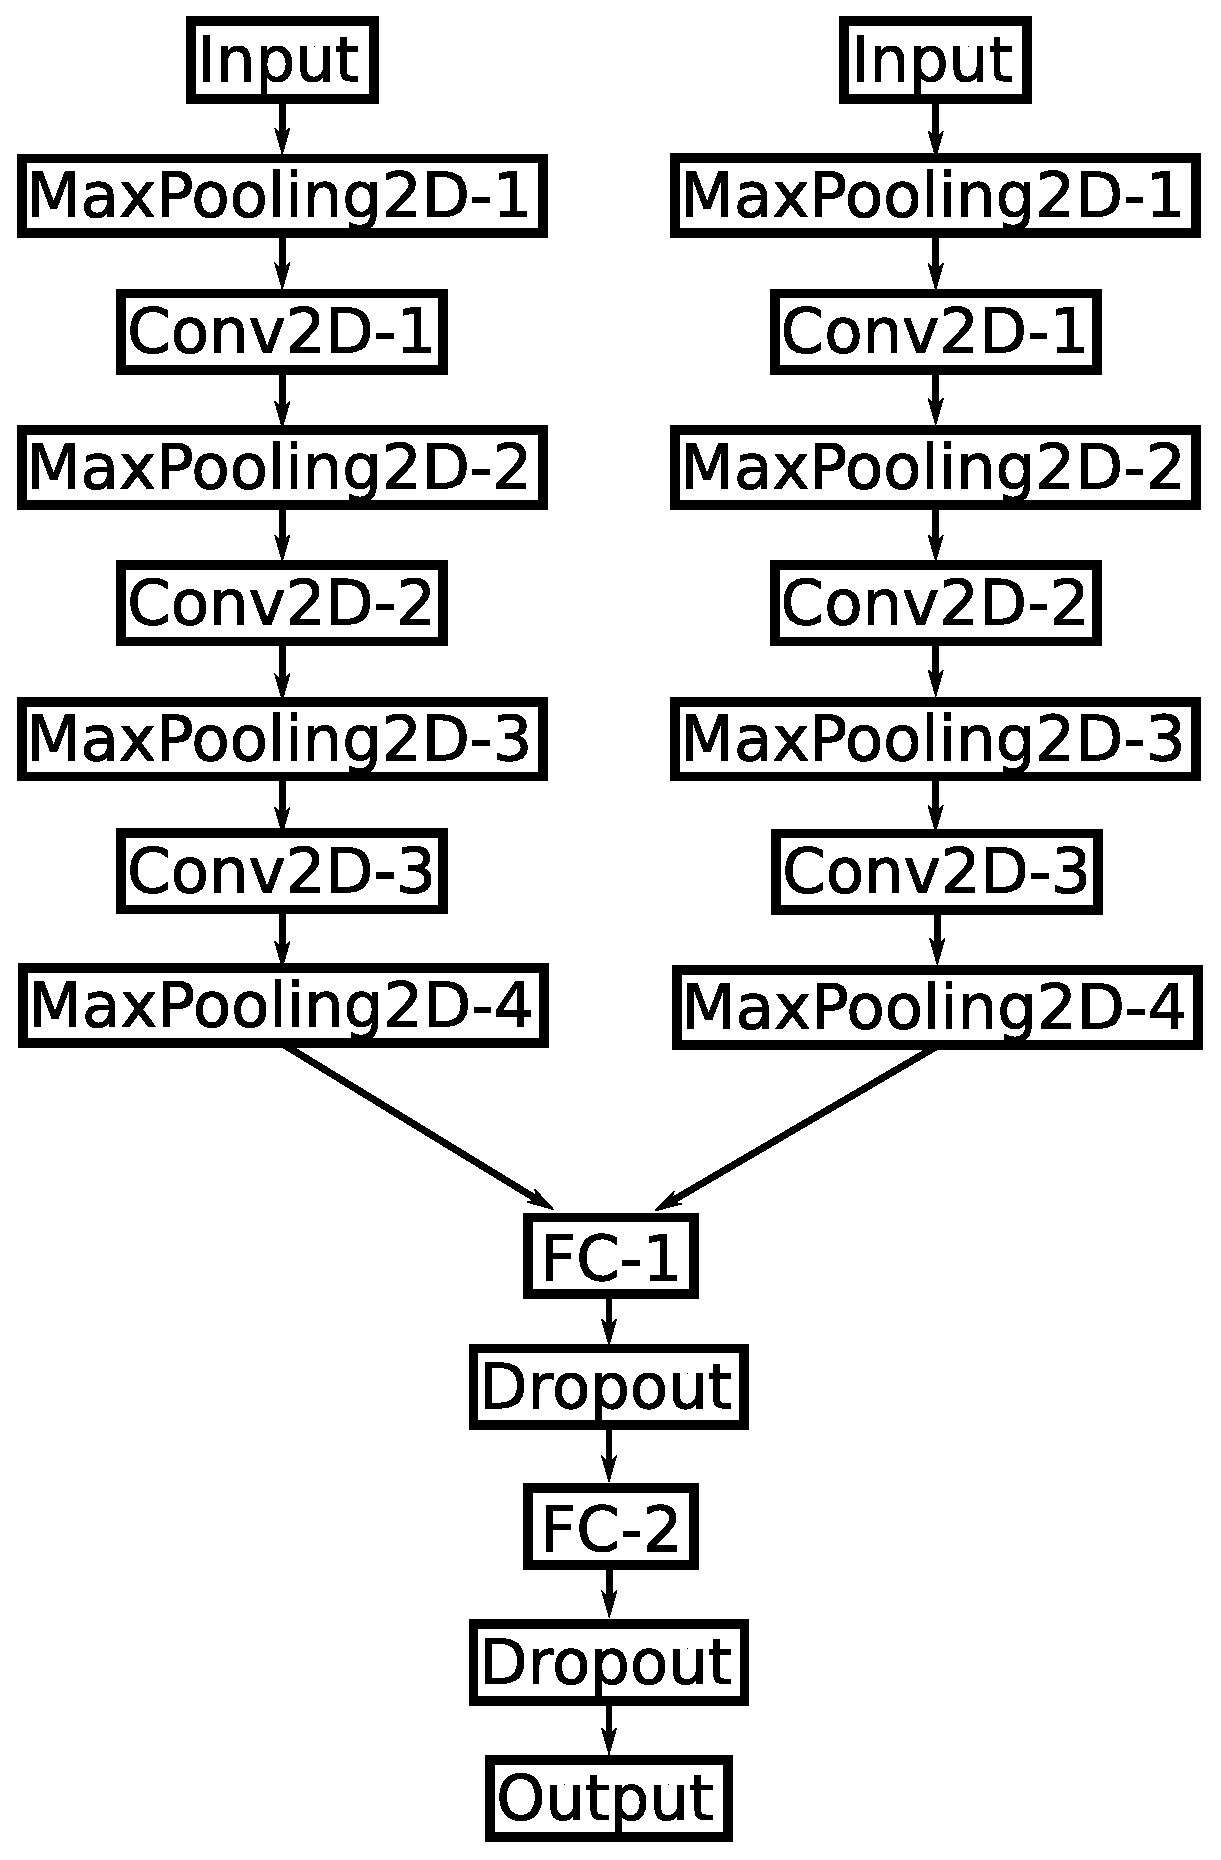
\includegraphics[clip, width=0.9\columnwidth]{eps/point_detection.eps}
    \caption{画像から情報を抽出するためのニューラルネットワーク}
    \label{fig:extraction}
  \end{minipage}
\end{figure}

MAIKo TPC から得られるデータが画像であるため、画像認識に有用とされるConvolutional Neural Network (CNN) を用いた。
CNN とはネットワーク内に畳み込み層を有するネットワーク構造である。
解析には事象の選別と飛跡情報の抽出の2つの段階があるため、
2種類のニューラルネットワークを用いて解析を行った。
事象の選別を行うニューラルネットワークと
画像から飛跡情報を抽出するニューラルネットワークの構造を
それぞれFig. \ref{fig:selection}とFig. \ref{fig:extraction}に示す。

事象選別のためのニュラルネットワークは、MAIKo TPC から得られる2つの画像を入力し、
その事象が標的と散乱した事象である確率を出力する。
出力された確率がある値以上である場合にその事象を標的と散乱した事象であると判断する。
anode image と cathode image では異なる特徴を持つため、
2つの入力が別れた構造を持つネットワークを構築した。
人間が判断したデータを用いて、学習および評価を行った。
学習には2,700 events、評価には300 events を使用した。

飛跡情報を抽出するためのネットワークには、
事象選別のときと同様に MAIKo TPC から得られる2つの飛跡画像を入力し、
散乱が起こった座標と反跳した${}^{4}\rm{He}$が停止した座標を出力させる。
%学習を効率的に行うために、出力される座標は各軸が0--1の範囲になるように規格化した座標系で得られる。
%このネットワークは21層からなり、2入力1出力の形をしている。
教師データには従来手法で決定した座標を用いた。
学習には3,012 events、評価には1,554 events を使用した。

学習環境はIntel Core i7、Nvidia GeForce GTX 1080Ti、Ubuntu 18.04 LTS、
TensorFlow~\cite{tensorflow}+Keras~\cite{keras} を用いた。

\section{Result}
\begin{wrapfigure}{r}{25zw}
  \vspace{-4zw}
  \centering
  \includegraphics[clip, width=25zw]{eps/point_detection_compair.eps}
  \caption{ニューラルネットワークによって決定した座標とHough変換によって決定した座標との比較}
  \label{fig:result_detection}
\end{wrapfigure}

事象選別のためのニューラルネットワークは、2,700 events に対して200 回学習を行った。
学習にはおよそ26分、その後の推測には300 events に対しておよそ1秒かかった。
従来手法の評価に用いたのと同じ実験データのうち、300 eventsを用いて評価を行った結果、
正解率は96\%であった。
従来の手法と比較して高精度に事象選別を行うことが可能となった。
また、パラメータチューニングおよび選別に要する時間も大きく短縮することができた。

座標の決定のためのニューラルネットワークは、3,012 events に対して500 回学習を行った。
学習にはおよそ270分、その後の推測には1,554 events に対しておよそ2秒かかった。
学習後にニューラルネットワークが予測した座標と従来手法によって決定した座標の比較をFig. \ref{fig:result_detection} に示す。
赤色の点は散乱が起こった点、緑色は反跳粒子が停止した点を表す。
丸点は従来型の手法を用いて決定した点 (学習に用いたデータ) 、
バツ点はニューラルネットワークを用いて決定した点を表す。
従来手法とニューラルネットワークを用いた手法のそれぞれで決定した座標は、
ほぼ一致している。
つまり、従来手法の精度を維持しつつ、
従来の手法と比較してパラメータチューニングおよび情報の抽出にかかる時間を短縮することができた。

\section{Conclusion}
従来のHough 変換を用いた画像識別アルゴリズムに変わる、
ニューラルネットワークを用いた新手法の開発を行った。
新手法は従来のものよりも高速かつ高精度に事象の選別を行うことが可能となった。
また、飛跡情報の抽出については従来の精度を保ちつつ、高速に行うことが可能となった。
ニューラルネットワークを用いた解析手法はTPC の解析に有用であることがわかった。

\begin{thebibliography}{9}
\bibitem{mupic}
  A.~Ochi, T.~Nagayoshi, T.~Tanimori, T.~Nagae, and M.~Nakamura
  Nuclear Instruments and Methods in Physics Research A \textbf{471} 264 (2001)
\bibitem{MAIKo}
  T.~Furuno, T.~Kawabata, H.~Ong, S.~Adachi, Y.~Ayyad, T.~Baba, Y.~Fujikawa, T.~Hashimoto, K.~Inaba, Y.~Ishii,
  S.~Kabuki, H.~Kubo, Y.~Matsuda, Y.~Matsuoka, T.~Mizumoto, T.~Morimoto, M.~Murata, T.~Sawano, T.~Suzuki, A.~Takada,
  J.~Tanaka, I.~Tanihata, T.~Tanimori, D.~Tran, M-, Tsumura, and H.~Watanabe
  Nuclear Instruments and Methods in Physics Research A \textbf{908} 215 (2018)
\bibitem{tensorflow}
  A.~Davis, J.~Dean, M.~Devin, S.~Ghemawat, I.~Goodfellow, A.~Harp, G.~Irving,
  M.~Isard, Y.~Jia, R.~Jozefowicz, L.~Kaiser, M.~Kudlur, J.~Levenberg,
  D.~Man\'{e}, R.~Monga, S.~Moore, D.~Murray, C.~Olah, M.~Schuster, J.~Shlens,
  B.~Steiner, I.~Sutskever, K.~Talwar, P.~Tucker, V.~Vanhoucke, V.~Vasudevan,
  F.~Vi\'{e}gas, O.~Vinyals, P.~Warden, M.~Wattenberg, M.~Wicke, Y.~Yu, and
  X.~Zheng, (2015).
  \url{https://tensorflow.org}
\bibitem{keras}
  F.~Chollet, et al. (2015). \url{https://keras.io}

%\bibitem{cp} The abbreviation for JPS Conference Proceedings should be ``JPS Conf. Proc." in the reference list.
%\bibitem{jpsj} The abbreviation for the Journal of the Physical Society of Japan should be ``J. Phys. Soc. Jpn." in the reference list.
%\bibitem{ptep} The abbreviation for the Progress of Theoretical and Experimental Physics should be ``Prog. Theor. Exp. Phys." in the reference list.
%\bibitem{instructions} More abbreviations of journal titles are listed in ``Instructions for Preparation of Manuscript", which is available at our Web site (http://jpsj.jps.or.jp).
%\bibitem{format} F. Author, S. Author, and T. Author, Abbreviated journal title \textbf{volume in bold face}, initial page or article number (year of publication).
\end{thebibliography}

\end{document}

